\documentclass[conference]{IEEEtran}
\IEEEoverridecommandlockouts
\usepackage{cite}
\usepackage{amsmath,amssymb,amsfonts}
\usepackage{algorithmic}
\usepackage{graphicx}
\usepackage{textcomp}
\usepackage{xcolor}
\usepackage{hyperref}
\usepackage{booktabs}
\usepackage{tikz}
\usetikzlibrary{shapes.geometric, arrows.meta, positioning, fit, backgrounds, shadows}
\def\BibTeX{{\rm B\kern-.05em{\sc i\kern-.025em b}\kern-.08em
    T\kern-.1667em\lower.7ex\hbox{E}\kern-.125emX}}

\begin{document}

\title{MarketFish: A Dual-LLM Agent-Based Social Media Simulation Engine with Algorithmic Seeding}

\author{\IEEEauthorblockN{Anonymous Authors}
\IEEEauthorblockA{\textit{Isal-NLP Laboratory} \\
City, Country \\
email@domain.com}
}

\maketitle

\begin{abstract}
Simulating social media dynamics is a critical challenge for computational sociology and digital marketing. Traditional Agent-Based Modeling (ABM) lacks the semantic nuance of real human interaction, while using Large Language Models (LLMs) for thousands of agents is often prohibitively expensive and prone to rate limits. In this paper, we introduce \textbf{MarketFish}, a highly scalable social media simulation engine utilizing a \textbf{Hybrid Agent-Based Modeling (Hybrid ABM)} architecture. MarketFish integrates a small subset of fully cognitive LLM agents (representing Key Opinion Leaders or KOLs) with a vast population of stochastic mathematical agents (representing the general public). Furthermore, we address the "Cold Start" bias through a Dual-Memory system backed by Retrieval-Augmented Generation (RAG), and simulate modern platform exposure using an FYP (For You Page) algorithmic seeder alongside KOL direct injection. Finally, we introduce an Astroturfing (Information Operations) simulation module to study the resilience of brand sentiment against coordinated bot attacks. Empirical observations from our asynchronous Python implementation demonstrate high throughput without hitting API rate limits, providing real-time analytical metrics such as Sentiment Timelines and Engagement Mixes via a WebSocket-driven React dashboard.
\end{abstract}

\begin{IEEEkeywords}
Agent-Based Modeling, Large Language Models, Social Media Simulation, Retrieval-Augmented Generation, Digital Marketing, FastAPI, WebSockets
\end{IEEEkeywords}

\section{Introduction}
The landscape of digital marketing on social platforms such as X (formerly Twitter), TikTok, and Facebook is highly volatile. A single campaign can trigger massive viral success or devastating public backlash ("cancel culture") within hours. Predicting these outcomes is notoriously difficult because it relies on complex network effects, algorithmic recommendations, and the unpredictable emotional responses of diverse demographic groups \cite{b1}.

Traditional Agent-Based Modeling (ABM) has been used to study opinion dynamics, but rule-based agents fail to capture the semantic and cultural nuances of modern internet slang and sarcasm. Recently, Generative AI and Large Language Models (LLMs) have been introduced to create autonomous persona-driven agents. However, simulating thousands of LLM-backed agents introduces severe architectural bottlenecks: exorbitant API costs, strict rate limits, and the "Cold Start" problem where agents lack pre-existing biases toward a brand \cite{b2}.

To solve these challenges, we propose \textbf{MarketFish}, a highly optimized Hybrid ABM simulation engine. Our contributions are fourfold:
\begin{enumerate}
    \item A \textbf{Hybrid ABM Architecture} that combines cognitive LLM agents with computationally lightweight mathematical agents, drastically reducing API costs while retaining emergent semantic behaviors.
    \item A \textbf{Dual-Memory RAG system} utilizing ChromaDB to solve the Cold Start problem, enabling agents to retain historical brand biases.
    \item An advanced \textbf{Algorithmic Injection Strategy} that models modern For You Page (FYP) discovery mechanisms and direct KOL seeding.
    \item An \textbf{Information Operations (IO) Simulator} designed to test brand resilience against coordinated astroturfing and bot attacks.
\end{enumerate}

\section{Methodology and System Architecture}

MarketFish is built upon an asynchronous pipeline designed to handle concurrent processing of thousands of agents. The architecture is divided into three core layers.

\begin{figure}[htbp]
\centering
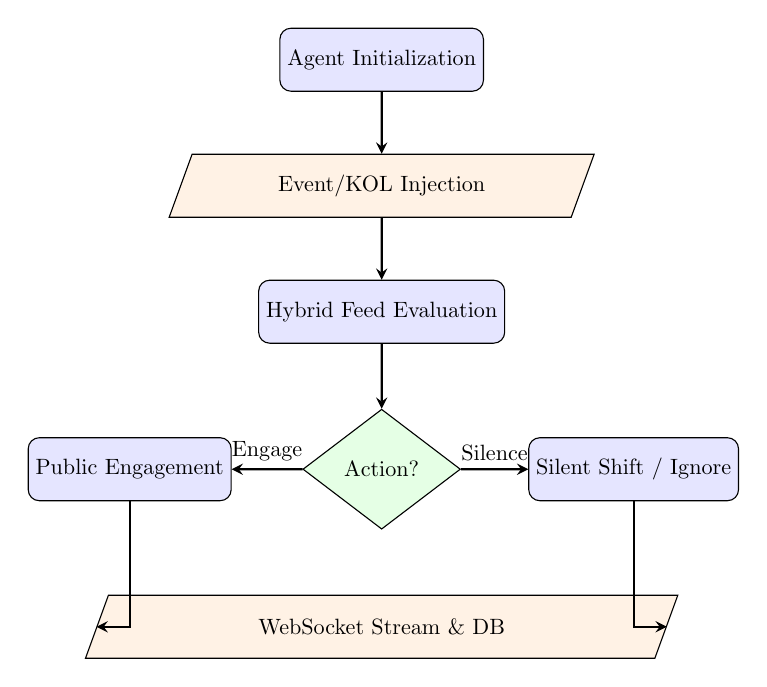
\begin{tikzpicture}[node distance=1.5cm, auto, scale=0.8, transform shape]
\tikzstyle{process} = [rectangle, minimum width=2.5cm, minimum height=1cm, text centered, draw=black, fill=blue!10, rounded corners]
\tikzstyle{io} = [trapezium, trapezium left angle=70, trapezium right angle=110, minimum width=2cm, minimum height=1cm, text centered, draw=black, fill=orange!10]
\tikzstyle{decision} = [diamond, minimum width=2.5cm, minimum height=1cm, text centered, draw=black, fill=green!10]
\tikzstyle{arrow} = [thick,->,>=stealth]

\node (init) [process] {Agent Initialization};
\node (event) [io, below of=init, yshift=-0.5cm] {Event/KOL Injection};
\node (feed) [process, below of=event, yshift=-0.5cm] {Hybrid Feed Evaluation};
\node (decision) [decision, below of=feed, yshift=-1cm] {Action?};
\node (public) [process, left of=decision, xshift=-2.5cm] {Public Engagement};
\node (silent) [process, right of=decision, xshift=2.5cm] {Silent Shift / Ignore};
\node (log) [io, below of=decision, yshift=-1cm] {WebSocket Stream \& DB};

\draw [arrow] (init) -- (event);
\draw [arrow] (event) -- (feed);
\draw [arrow] (feed) -- (decision);
\draw [arrow] (decision) -- node[anchor=south] {Engage} (public);
\draw [arrow] (decision) -- node[anchor=south] {Silence} (silent);
\draw [arrow] (public) |- (log);
\draw [arrow] (silent) |- (log);
\end{tikzpicture}
\caption{MarketFish Pipeline Workflow Diagram illustrating the agent evaluation lifecycle.}
\label{fig:pipeline}
\end{figure}

\subsection{Hybrid Agent-Based Modeling (Hybrid ABM)}
To balance cognitive depth with computational cost, the engine decouples the agent population into two distinct tiers:
\begin{itemize}
    \item \textbf{Cognitive Agents (KOLs):} A precise subset of agents (typically 1-5\% of the population) are powered by the \textit{Qwen-3.7-flash} model. These agents possess complete linguistic reasoning, generate context-aware comments, and synthesize complex sentiments.
    \item \textbf{Stochastic Mathematical Agents (The Public):} The vast majority of the population (95\%+) is simulated using a lightweight mathematical model. These agents react based on the prevailing \textit{Sentiment Trend} established by the Cognitive Agents. Their reaction probabilities are defined by a logistic function influenced by demographic weighting and pre-existing biases, allowing the system to scale to hundreds of thousands of agents with near-zero computational overhead.
\end{itemize}

\subsection{Astroturfing and Information Operations (IO)}
Social media platforms are frequently manipulated by coordinated inauthentic behavior. MarketFish introduces an IO module that allocates a configurable percentage of the mathematical agents as ``Bots''. These bots forcefully inject predefined extreme sentiments (either artificially positive praise or coordinated negative attacks) into the simulation. This allows marketers to observe the organic population's resilience and polarization when subjected to artificial echo chambers.

\subsection{Memory and the Cold Start Problem}
A significant flaw in zero-shot LLM agents is their lack of historical bias. If an agent is spawned to review a post from a historically controversial brand, a blank-slate agent will react neutrally, reducing simulation realism.

MarketFish utilizes a \textbf{Dual-Memory System}:
\begin{enumerate}
    \item \textbf{Short-Term Memory (Redis):} Holds immediate contextual interactions during an active simulation tick.
    \item \textbf{Long-Term Memory (ChromaDB):} Stores vectorized historical data. To solve the Cold Start problem, we inject \textit{Scraped Real-World Data} into ChromaDB via RAG. Agents query this database to retrieve authentic past sentiments regarding the brand before reacting to new campaigns.
\end{enumerate}

\subsection{Topology and FYP Algorithmic Seeding}
Information on modern social networks does not propagate solely through social graphs (followers). Recommendation algorithms (e.g., TikTok's For You Page) expose content to strangers based on engagement metrics. 

Our Orchestrator simulates this by initiating \textbf{Tick 1 (FYP Seeding)}, where content is algorithmically injected to the observation queues of $N$ random agents outside the brand's network. Alternatively, the system allows for \textbf{KOL Injection}, bypassing the FYP algorithm entirely to seed content directly into the feeds of the most influential Cognitive Agents.

Subsequent ticks ($T > 1$) utilize a Small-World Network topology to propagate shared content to second-degree connections. The probability of an agent $i$ seeing a post at time $T$ is given by:
\begin{equation}
P(S_{i, T}) = \alpha \cdot FYP(i) + (1 - \alpha) \cdot \sum_{j \in N(i)} W_{j,i} Share(j, T-1)
\end{equation}
where $FYP(i)$ is the algorithmic exposure, $N(i)$ is the neighbor set, and $W_{j,i}$ is the edge weight between agents. If the overall engagement rate exceeds a viral threshold (e.g., $\tau > 15\%$), the algorithm triggers secondary FYP waves, pushing the content to previously unreached demographic clusters.

\begin{figure*}[t]
\centering
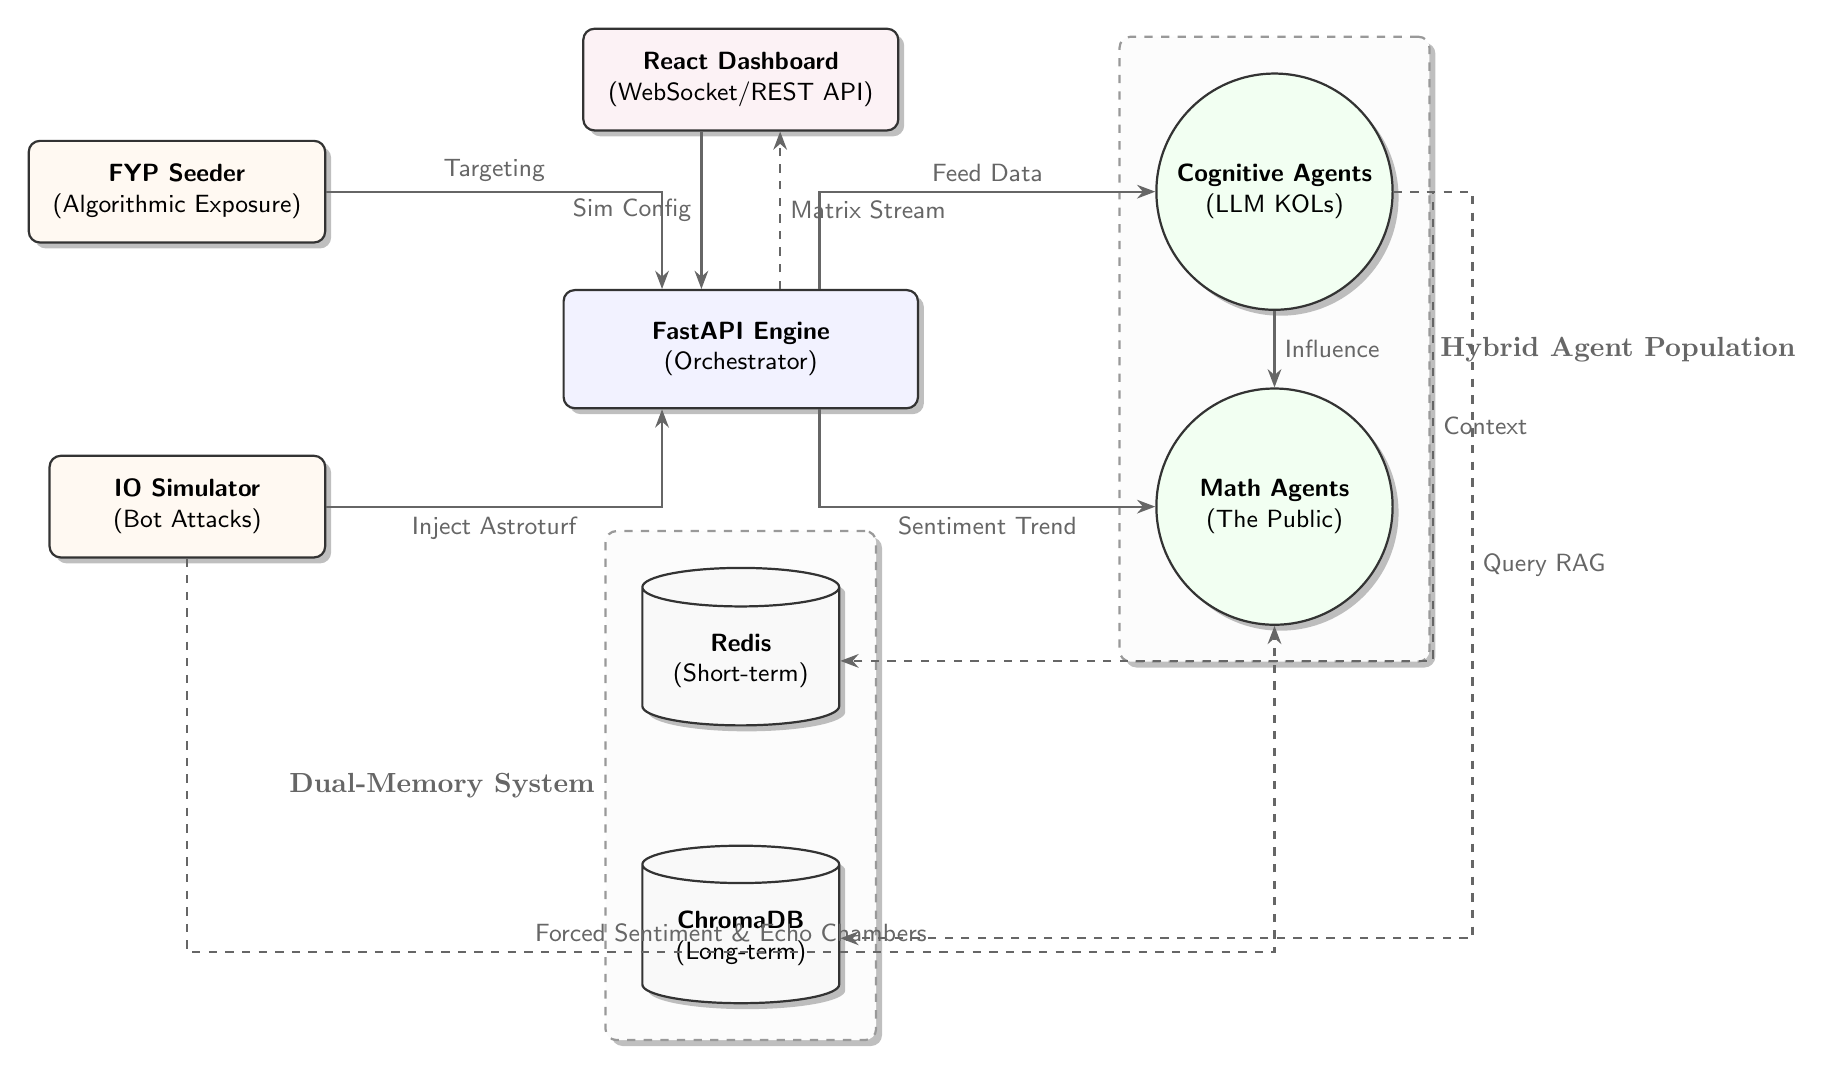
\begin{tikzpicture}[
    node distance=1.5cm and 2.5cm,
    font=\sffamily\small,
    >=Stealth,
    base/.style={draw=black!80, rounded corners, align=center, inner sep=2ex, thick, drop shadow},
    frontend/.style={base, fill=purple!5, minimum width=4cm},
    core/.style={base, fill=blue!5, minimum width=4.5cm, minimum height=1.5cm},
    injector/.style={base, fill=orange!5, minimum width=3.5cm},
    db/.style={cylinder, shape border rotate=90, aspect=0.25, draw=black!80, thick, align=center, fill=gray!5, minimum width=2.5cm, minimum height=2cm, drop shadow},
    agent/.style={circle, draw=black!80, thick, align=center, fill=green!5, minimum size=3cm, drop shadow},
    groupbox/.style={draw=black!40, dashed, thick, rounded corners, inner sep=3ex, fill=gray!2, drop shadow},
    arrow/.style={->, thick, color=gray!80!black},
    dashed_arrow/.style={->, thick, dashed, color=gray!80!black}
]

% Middle Column
\node[core] (api) {\textbf{FastAPI Engine}\\(Orchestrator)};
\node[frontend, above=2cm of api] (dashboard) {\textbf{React Dashboard}\\(WebSocket/REST API)};
\node[db, below=2cm of api] (redis) {\textbf{Redis}\\(Short-term)};
\node[db, below=1.5cm of redis] (chroma) {\textbf{ChromaDB}\\(Long-term)};

% Left Column
\node[injector, left=3cm of api, yshift=2cm] (fyp) {\textbf{FYP Seeder}\\(Algorithmic Exposure)};
\node[injector, left=3cm of api, yshift=-2cm] (io) {\textbf{IO Simulator}\\(Bot Attacks)};

% Right Column
\node[agent, right=3cm of api, yshift=2cm] (llm) {\textbf{Cognitive Agents}\\(LLM KOLs)};
\node[agent, right=3cm of api, yshift=-2cm] (math) {\textbf{Math Agents}\\(The Public)};

% Group Boxes
\begin{scope}[on background layer]
    \node[groupbox, fit=(chroma) (redis), label={[font=\bfseries, color=gray!80!black]left:Dual-Memory System}] (memorybox) {};
    \node[groupbox, fit=(llm) (math), label={[font=\bfseries, color=gray!80!black]right:Hybrid Agent Population}] (agentbox) {};
\end{scope}

% Connections
% Dashboard <-> API
\draw[arrow] (dashboard.south) ++(-0.5,0) -- node[left] {Sim Config} ([xshift=-0.5cm]api.north);
\draw[dashed_arrow] ([xshift=0.5cm]api.north) -- node[right] {Matrix Stream} ([xshift=0.5cm]dashboard.south);

% Inputs -> API
\draw[arrow] (fyp.east) -| node[near start, above] {Targeting} ([xshift=-1cm]api.north);
\draw[arrow] (io.east) -| node[near start, below] {Inject Astroturf} ([xshift=-1cm]api.south);

% API -> Agents
\draw[arrow] ([xshift=1cm]api.north) |- node[near end, above] {Feed Data} (llm.west);
\draw[arrow] ([xshift=1cm]api.south) |- node[near end, below] {Sentiment Trend} (math.west);

% Memory Interactions
\draw[dashed_arrow] (llm.east) -- ++(0.5,0) |- node[near start, right] {Context} (redis.east);
\draw[dashed_arrow] (llm.east) -- ++(1.0,0) |- node[near start, right] {Query RAG} (chroma.east);

% Agent Interactions
\draw[arrow] (llm.south) -- node[right] {Influence} (math.north);

% IO to Math directly
\draw[dashed_arrow] (io.south) -- ++(0,-5cm) -| node[near start, above] {Forced Sentiment \& Echo Chambers} (math.south);

\end{tikzpicture}
\caption{Comprehensive MarketFish Architecture Diagram: Illustrating the integration between the orchestration layer, Dual-Memory system (ChromaDB/Redis), and the Hybrid Agent population.}
\label{fig:detailed_arch}
\end{figure*}

\section{Implementation Details}
The MarketFish engine is implemented as a Full-Stack application:
\begin{itemize}
    \item \textbf{Backend Engine:} Built in Python using \texttt{FastAPI} and \texttt{asyncio}. Concurrency is strictly managed using \texttt{asyncio.Semaphore} to prevent LLM API rate limit explosion during viral bursts.
    \item \textbf{Frontend Dashboard:} A premium React application utilizing \texttt{Recharts} for dynamic data visualization. It connects to the backend via REST for configuration and WebSockets for a real-time \textit{Matrix Feed}, streaming simulated agent comments dynamically. 
\end{itemize}

\section{Discussion and Evaluation}
Our preliminary trials indicate that the Hybrid ABM approach preserves the emergent properties of complex social systems without incurring exponential API costs. The inclusion of mathematical agents driven by LLM-generated sentiment trends successfully replicates the "herd mentality" observed in real-world social networks.

Furthermore, the advanced analytics dashboard computes a continuous \textbf{Sentiment Timeline} and \textbf{Engagement Mix}, providing marketers with granular, tick-by-tick visibility into public perception. When subjected to the Negative IO simulation, the system accurately modeled a viral crisis, demonstrating the platform's efficacy as a stress-testing environment for digital PR campaigns.

\section{Conclusion and Future Work}
MarketFish demonstrates that simulating massive, highly realistic social media environments is both technically feasible and economically viable using a Dual-LLM architecture and clustered demographic grouping. Future work will focus on integrating automated clustering pipelines (K-Means on BGE-M3 embeddings) to classify unlabeled scraped social data directly into generational archetypes for the RAG database.

\begin{thebibliography}{00}
\bibitem{b1} C. Bail, ``Breaking the Social Media Prism: How to Make Our Platforms Less Polarizing,'' Princeton University Press, 2021.
\bibitem{b2} J. S. Park, J. C. O'Brien, C. J. Cai, M. R. Morris, P. Liang, and M. S. Bernstein, ``Generative Agents: Interactive Simulacra of Human Behavior,'' in \textit{Proc. of the 36th Annual ACM Symposium on User Interface Software and Technology (UIST)}, 2023.
\bibitem{b3} A. Vaswani et al., ``Attention is All You Need,'' \textit{Advances in Neural Information Processing Systems}, vol. 30, 2017.
\end{thebibliography}

\end{document}
